% Chapter Template

\chapter{Approximation of CLT Based on Artificial Neural Network} % Main chapter title

\label{Chapter5} % Change X to a consecutive number; for referencing this chapter elsewhere, use \ref{ChapterX}

%----------------------------------------------------------------------------------------
%	SECTION 1
%----------------------------------------------------------------------------------------

\section{Neural Network Design}
Artificial neural networks(ANN) which heavily inspired by biology and psychology
have been widely used to solve various practical engineering problems in such
areas as pattern recognition, nonlinear regression, data mining, clustering and
prediction. Methods based on complicated mathematical models is of intensive
computation, approximation function evaluation techniques can be employed to
accelerate the calculation process and reduce the computation cost. In order to
solve practical engineering problems in composite material application, classic
laminational theory(CLT) has been proposed which involves many matrix
multiplication and integration calculation. ANN which has been proved is a
reliable tool instead of complicate mathematical model.  The design of neural
network consists of three basic parts: neural network architecture, learning
rules, and training techniques.

The weight training in ANN is to minimize the error function, such as the most
widely used mean square error which calculate the difference  between the
desired and the prediction output values averaged over all examples.
Backpropation algorithm has been successful applied to in many areas, and it's
based on gradient descent. However, this class of algorithms are  plagued by the
possible existance of local minima or "flat spots" and "the curse of
dimensionality". One method to overcome this problem is to adopt EANN's 

\subsection{Architecture}
The inputs of the neural network is consist of four parts: in-plane loading
$N_x$, $N_y$, and $N_{xy}$, design parameters of laminate, two distinct fiber
orientation angle $\theta_1$ and $\theta_2$, ply thickness $t$, total number of
plies $N$; five engineering constants of composite materials, $E_1$, $E_2$, ;
five strength parameters of a unidirectional lamina. There are two outputs in
the neural network, safety factors for MS theory and Tsai-Wu theory, respectively.

\begin{figure}
	\begin{center}
\begin{tikzpicture}
[ plain/.style={ draw=none, fill=none, }, remember picture, net/.style={ matrix of nodes, nodes={ draw, circle,
    inner sep=7.5pt
    },
  nodes in empty cells,
  column sep=-10.5pt,
  row sep=0.8cm
  }
]
%\draw[help lines] (-3cm,-6cm) grid (6cm,3cm);
\matrix[net] (mat)
{
              & |[plain]| &           & |[plain]|  &           & |[plain]| &           &  |[plain]|      &               \\
    |[plain]| &           & |[plain]| &            & |[plain]| &           & |[plain]| &                 & |[plain]|     \\ 
    |[plain]| & |[plain]| &           & |[plain]|  &           & |[plain]| & 	  	   &  |[plain]|      & |[plain]|     \\ 
  };

  \node at ($(mat-1-1.west)+(-16pt,0)$) {Input: };
  \node at ($(mat-2-2.west)+(-24pt,0)$) {Hidden:};
  \node at ($(mat-3-2.west)+(-24pt,0)$) {Output:};
  \node at (mat-1-1.base) {$i_1$};
  \node at (mat-1-3.base) {$i_2$};
  \node at (mat-1-5.base) {...};
  \node at (mat-1-7.base) {$i_{n-1}$};
  \node at (mat-1-9.base) {$i_{n}$};
  \node at (mat-2-2.base) {$h_1$};
  \node at (mat-2-4.base) {$h_2$};
  \node at (mat-2-6.base) {$...$};
  \node at (mat-2-8.base) {$h_{m}$};
  \node at (mat-3-5.base) {$...$};

 \foreach \a in {1,3}{
    \foreach \b in {2,6}{
        \draw[->] (mat-1-\a.south) -- (mat-2-\b.north);
     }
  }
 \foreach \a in {3,7,9}{
    \foreach \b in {4,8}{
        \draw[->] (mat-1-\a.south) -- (mat-2-\b.north);
     }
  }

 \foreach \c in {2,4,6,8}{
    \foreach \d in {3,5,7}{
 		\draw[->] (mat-2-\c.south) -- (mat-3-\d.north);
	}
 }
\end{tikzpicture}
\caption{Neural Network Model}
\end{center}
\end{figure}

\begin{figure}
\centering
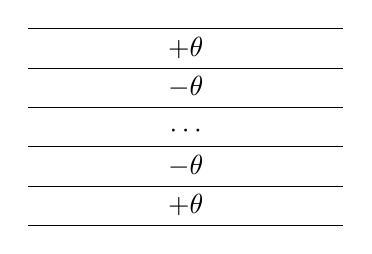
\begin{tikzpicture}
	\draw (0,0) -- (4,0);
	\draw (0,-0.5) -- (4,-0.5) node[midway, above] {$\mathit{+}\theta$};
	\draw (0,-1) -- (4,-1) node[midway, above] {$\mathit{-}\theta$} ;
	\draw (0,-1.5) -- (4,-1.5) node[midway, above] {$\cdots$};
	\draw (0,-2) -- (4,-2) node[midway, above] {$\mathit{-}\theta$};
	\draw (0,-2.5) -- (4,-2.5) node[midway, above] {$\mathit{+}\theta$};
\end{tikzpicture}
\caption{Model for Angle ply laminate}
\end{figure}


\begin{figure*}
\centering
\begin{tikzpicture}
[ p/.style={ draw=none, fill=none, }, remember picture, 
  net/.style={ matrix of nodes, nodes={ draw, circle, inner sep=7.5pt },
  nodes in empty cells,
  column sep=-10.5pt,
  row sep=0.8cm
  }
]
%\draw[help lines] (-3cm,-6cm) grid (6cm,3cm);
\matrix[net] (mat)
{
	  & |[p]| &  & |[p]| &  & |[p]| &  & |[p]| &  & |[p]| &  & |[p]| &  & |[p]| &  & |[p]| &  &
	    |[p]| &  & |[p]| &  & |[p]| &  & |[p]| &  & |[p]| &  & |[p]| &  & |[p]| &  & |[p]|    \\
 |[p]| & |[p]| & |[p]| &  |[p]| &        & |[p]| & |[p]| & |[p]| &|[p]| &       & |[p]| &  |[p]| & |[p]| &
 |[p]| &       & |[p]| &  |[p]| &  |[p]| & |[p]| & |[p]| &       &|[p]| & |[p]| & |[p]| & |[p]|
	   & |[p]| &       &  |[p]| &  |[p]| & |[p]| & |[p]| & |[p]| &|[p]| \\ 
 |[p]| &  |[p]| & |[p]|  &  |[p]| & |[p]|  &  |[p]| &  |[p]| &  |[p]| & |[p]| & |[p]| & |[p]| &       & |[p]|
	   &  |[p]| & |[p]|  &  |[p]| &        &  |[p]| &  |[p]| &  |[p]| & |[p]| & |[p]| & |[p]| & |[p]| &     |[p]|
	   &  |[p]| & |[p]|  &  |[p]| & |[p]|  &  |[p]| &  |[p]| &  |[p]| \\ 
  };
  \draw[<-] (mat-1-1.north) --  ++(0,1) node {$N_x$};
  \draw[<-] (mat-1-3.north) --  ++(0,1) node {$N_y$};
  \draw[<-] (mat-1-5.north) --  ++(0,1) node {$N_{xy}$};
  \draw[<-] (mat-1-7.north) --  ++(0,1) node {$\theta_1$};
  \draw[<-] (mat-1-9.north) --  ++(0,1) node {$\theta_2$};
  \draw[<-] (mat-1-11.north) --  ++(0,1) node {$t$};
  \draw[<-] (mat-1-13.north) --  ++(0,1) node {$N$};
  \draw[<-] (mat-1-15.north) --  ++(0,1) node {$E_1$};
  \draw[<-] (mat-1-17.north) --  ++(0,1) node {$E_2$};
  \draw[<-] (mat-1-19.north) --  ++(0,1) node {$G_{12}$};
  \draw[<-] (mat-1-21.north) --  ++(0,1) node {$v_{12}$};
  \draw[<-] (mat-1-23.north) --  ++(0,1) node {$\sigma_1^T$};
  \draw[<-] (mat-1-25.north) --  ++(0,1) node {$\sigma_1^C$};
  \draw[<-] (mat-1-27.north) --  ++(0,1) node {$\sigma_2^T$};
  \draw[<-] (mat-1-29.north) --  ++(0,1) node {$\sigma_2^C$};
  \draw[<-] (mat-1-31.north) --  ++(0,1) node {$\tau_{12}$};
  \draw[->] (mat-3-12.south) --  ++(0,-1) node[pos=0.5, swap] {Tsai-Wu};
  \draw[->] (mat-3-17.south) --  ++(0,-1) node[pos=0.5, swap] {MS};
  \node at ($(mat-1-1.west)+(-16pt,0)$) {Input: };
  \node at ($(mat-2-2.west)+(-24pt,0)$) {Hidden:};
  \node at ($(mat-3-2.west)+(-24pt,0)$) {Output:};
  \node at (mat-2-5.base) {$h_1$};
  \node at (mat-2-10.base) {$h_2$};
  \node at (mat-2-15.base) {$...$};
  \node at (mat-2-21.base) {\small{$h_{m-1}$}};
  \node at (mat-2-27.base) {$h_{m}$};
 \foreach \a in {1,3,5,7,9,11,31}{
        \draw[->] (mat-1-\a.south) -- (mat-2-5.north);
     }
 \foreach \a in {5,7,11,19,25,27}{
        \draw[->] (mat-1-\a.south) -- (mat-2-10.north);
     }
 \foreach \a in {1,7,11,17,19,25}{
        \draw[->] (mat-1-\a.south) -- (mat-2-15.north);
     }
 \foreach \a in {5,9,19,21,29}{
        \draw[->] (mat-1-\a.south) -- (mat-2-21.north);
     }
 \foreach \a in {11,15,19,23,27,29,31}{
        \draw[->] (mat-1-\a.south) -- (mat-2-27.north);
     }
 \foreach \c in {5,10,15,21,27}{
    \foreach \d in {12,17}{
 		\draw[->] (mat-2-\c.south) -- (mat-3-\d.north);
	}
 }
\end{tikzpicture}
\caption{Neural Network Model}
\end{figure*}


\section{Approximation Framework}
\subsection{Data Preparation}
\begin{table}	
	\begin{tabular}{cccc|cc}
		\toprule
		\multicolumn{4}{c}{\textbf{Input}} &  \multicolumn{2}{c}{\textbf{Output}} \\
		\midrule
		Load  &  Laminate  & Material & Failure  & MS & Tsai-Wu \\
		      &  Structure & Property & Property &    &         \\
		\midrule
		\tiny{120,5,0} &  \tiny{10,-10,8,1.27} &  \tiny{38.6,8.27,0.26,4.14} &  \tiny{1062.0,610.0,31,118,72} &  \tiny{0.068} &\tiny{ 0.062}\\
		\tiny{120,5,0} &  \tiny{10,-10,2,1.27} &  \tiny{38.6,8.27,0.26,4.14} &  \tiny{1062.0,610.0,31,118,72} &  \tiny{1.69}  &\tiny{ 2.18}\\
		\tiny{...}     &   \tiny{...}          & \tiny{...}                  &  \tiny{...}                    &  \tiny{...}  &  \tiny{...}\\
		\tiny{120,5,0} &  \tiny{10,-10,134,1.27} &  \tiny{38.6,8.27,0.26,4.14} &  \tiny{1062.0,610.0,31,118,72} &  \tiny{1.70} &\tiny{1.56 }\\
		\tiny{120,5,0} &  \tiny{10,-10,8,1.27} &  \tiny{181,10.3,0.28,7.17} &  \tiny{1500.0,1500.0,40,246,68} &  \tiny{0.072} &\tiny{ 0.024}\\
		\bottomrule
		\end{tabular}
\end{table}

It's implausible to obatain the training data from practial experiments, so CLT
is taken to generate the training data and evaluation data. Three composite
materials are used, as shown in Table \ref{tab:mat}. The fiber orientation range
is from -90 to 90, the number of layers range is from 5 to 200. Assuming the
composite material only subjects to in-plane loading, each component range is
from -90 to 90;

we sample this function to yield 140000 points distributed uniformly over
aboved mentioned ranges as the training data.

\subsection{Training}
\afterpage{
\begin{figure}
		\centering
		\begin{tikzpicture}
			%\draw[help lines] (-3cm,-6cm) grid (6cm, 6cm);
			\tikzstyle{block} = [rectangle, text centered, draw=black,
			minimum width=1.1cm, minimum height=0.4cm]
			% first level
			\node (evaluation-parent) [block, minimum width=2.4cm, minimum
				height=1.8cm,draw=white] {};
			\node (evaluation) [block] at ($(evaluation-parent.north)$) {evaluation};
			\node (reproduction) [block] at ($(evaluation-parent.south)$) {reproduction};
			\node (tasks) [block, minimum width=1.1cm, minimum height=0.4cm] {tasks};

			\draw[->] ($(evaluation.south)+(0.3cm,0cm)$) --
				($(tasks.north)+(0.3cm,0cm)$) node[auto=left, pos=0.5] {\small weights}; 
			\draw[<-] ($(evaluation.south)+(-0.3cm,0cm)$) --
				($(tasks.north)+(-0.3cm,0cm)$) node[auto=right, pos=0.5] {\small fitness}; 

			% get intersection
			\draw[white] (evaluation.west) coordinate (A) -- ++(-1.5cm,0) coordinate (B);
			\draw[white] (reproduction.west) -- ++(-0.3cm,0) coordinate (C) -- ++(0,4cm) coordinate
						(D);
			\draw[black] (reproduction.west) -- ++(-0.3cm,0) -- (intersection cs:
				first line={(A)--(B)}, second line={(C)--(D)}) coordinate (E);
			\draw[->] (E) -- (evaluation.west);

			\draw[white] (evaluation.east) coordinate (E) -- ++(2cm,0) coordinate (F);
			\draw[white] (reproduction.east) -- ++(0.3cm,0) coordinate (G) -- ++(0,4cm) coordinate
				(H);
			\draw[<-] (reproduction.east) -- ++(0.3cm,0) -- (intersection cs:
				first line={(E)--(F)}, second line={(G)--(H)}) coordinate (I);
			\draw (I) -- (evaluation.east);

			% second level
			\node (level2) [block,draw=black, minimum width=3.5cm, minimum height=3.0cm] at
				(0cm,0.2cm) {};
			\node [align=left] at ($(level2.north)+(0,-0.2cm)$) {\tiny THE EVOLUTION
				OF};
			\node [align=left] at ($(level2.north)+(0,-0.45cm)$) {\tiny CONNECTION
					WEIGHTS 
				};
			% third level
			\node (level3-assister) [block, draw=white, minimum width=5cm, minimum
				height=4.6cm] at
				(0, 0.3cm)  {};
			\node (evaluation) [block] at ($(level3-assister.north)$) {\small evaluation of
				learning rules};
					\node (reproduction) [block] at ($(level3-assister.south)$) {\small reproduction of
				learning rules};

			\draw[->] ($(evaluation.south)+(0.3cm,0cm)$) --
				($(level2.north)+(0.3cm,0cm)$) node[auto=left, pos=0.5] {\small learning
				rule}; 
			\draw[<-] ($(evaluation.south)+(-0.3cm,0cm)$) --
				($(level2.north)+(-0.3cm,0cm)$) node[auto=right, pos=0.5] {\small fitness}; 

			\draw[white] (evaluation.west) coordinate (A) -- ++(-1.3cm,0) coordinate (B);
			\draw[white] (reproduction.west) -- ++(-0.3cm,0) coordinate (C) -- ++(0,4cm) coordinate
				(D);
			\draw[black] (reproduction.west) -- ++(-0.3cm,0) -- (intersection cs:
				first line={(A)--(B)}, second line={(C)--(D)}) coordinate (E);
			\draw[->] (E) -- (evaluation.west);

			\draw[white] (evaluation.east) coordinate (E) -- ++(2cm,0) coordinate (F);
			\draw[white] (reproduction.east) -- ++(0.3cm,0) coordinate (G) -- ++(0,4cm) coordinate
				(H);
			\draw[<-] (reproduction.east) -- ++(0.3cm,0) -- (intersection cs:
						first line={(E)--(F)}, second line={(G)--(H)}) coordinate (I);
			\draw (I) -- (evaluation.east);
		   % fourth level
			\node (level4) [block, draw=black, minimum width=5.5cm, minimum
				height=6.0cm] at
				(0, 0.4cm)  {};
			\node [align=left] at ($(level4.north)+(0,-0.25cm)$) {\tiny THE EVOLUTION
				OF LEARNING RULES};
			% level five
			\node (level5-assister) [block, draw=white, minimum width=6.4cm, minimum
				height=7.0cm] at
				(0, 0.4cm)  {};
			\node (evaluation) [block] at ($(level5-assister.north)$) {\small evaluation of
				architecture};
			\node (reproduction) [block] at ($(level5-assister.south)$) {\small reproduction of
				learning architecture};

			\draw[white] (evaluation.west) coordinate (A) -- ++(-1.5cm,0) coordinate (B);
			\draw[white] (reproduction.west) -- ++(-0.6cm,0) coordinate (C) -- ++(0,4cm) coordinate
				(D);
			\draw[black] (reproduction.west) -- ++(-0.6cm,0) -- (intersection cs:
				first line={(A)--(B)}, second line={(C)--(D)}) coordinate (E);
			\draw[->] (E) -- (evaluation.west);

			\draw[white] (evaluation.east) coordinate (E) -- ++(2cm,0) coordinate (F);
			\draw[white] (reproduction.east) -- ++(0.6cm,0) coordinate (G) -- ++(0,4cm) coordinate
				(H);
			\draw[<-] (reproduction.east) -- ++(0.6cm,0) -- (intersection cs:
						first line={(E)--(F)}, second line={(G)--(H)}) coordinate (I);
			\draw (I) -- (evaluation.east);
			% level 6
			\node (level6) [block, minimum width=7.0cm, minimum
				height=8.1cm] at
				(0, 0.5cm)  {};
			\node [align=left] at ($(level6.north)+(0,-0.2cm)$) {\tiny THE EVOLUTION OF
					ARCHITECTURE
						};
			\end{tikzpicture}
		\caption{Genetic algorithm and artificial neural network}
\end{figure}
\clearpage
}


\subsection{Evaluation}
\begin{table}	
	\centering
	\caption{Comparsion between practical and simulation}
	\label{tab:simu}
		\resizebox{\textwidth}{!}{
	\begin{tabular}{cccc|cc|cc}
		\toprule
		\multicolumn{4}{c}{\textbf{Input}} &  \multicolumn{4}{c}{\textbf{Output}} \\
		\midrule
		Load  &  \makecell{Laminate \\ Structure }  & \makecell{Material \\ Property} & \makecell{Failure \\  Property}  &
		\multicolumn{2}{c}{ \makecell {CLT \\MS  Tsai-Wu}} & \multicolumn{2}{c}{ \makecell {ANN \\MS  Tsai-Wu}}\\
		\midrule
		-10,40,20  &  26,-26,168,1.27 & 116.6,7.67,0.27,4.17 & 2062.0,1701.0,70,240,105 & 0.342 & 0.476 & 0.351 & 0.492 \\
		20,-70,-30 &  10,-10,196,1.27 & 181.0,10.3,0.28,7.17 & 1500.0,1500.0,40,246,68  & 0.653 & 0.489 & 0.612 & 0.445 \\ 
		60,-20,0   &  82 -82,128,1.27 & 181.0,10.3,0.28,7.17 & 1500.0,1500.0,40,246,68  & 1.663 & 0.112 & 1.673 & 0.189 \\
		\bottomrule
	\end{tabular}
	}
\end{table}

\subsection{Result and Discussion}
\section{Summary}

